\documentclass[10pt]{article}
\usepackage[T1]{fontenc} \usepackage{amsmath}
\usepackage{amsfonts}
\usepackage{amssymb}
\usepackage{listings}
\usepackage[version=4]{mhchem}
\usepackage{bbold}
\usepackage{graphicx}
\usepackage[export]{adjustbox}
\usepackage{xcolor}
\usepackage{bbold}
\usepackage{soul}
\usepackage{tikz,pgfplots, lipsum,lmodern}
\usepackage[T1]{fontenc}
\usepackage[ngerman]{babel}
\usepackage{adigraph}
\pgfplotsset{compat=1.18, width=10cm}
\usetikzlibrary{positioning}

\usepackage{nicematrix,tikz}
\usepackage[tmargin=2cm,rmargin=1in,lmargin=1in,margin=0.85in,bmargin=2cm,footskip=.2in]{geometry}
\usepackage{amsmath,amsfonts,amsthm,amssymb,mathtools}
\usepackage[varbb]{newpxmath}
\usepackage{xfrac}
\usepackage[makeroom]{cancel}
\usepackage{mathtools}
\usepackage{bookmark}
\usepackage{enumitem}
\usepackage[most,many,breakable]{tcolorbox}
\usepackage{varwidth}
\usepackage{varwidth}
\usepackage{etoolbox}
%\usepackage{authblk}
\usepackage{nameref}
\usepackage{multicol,array}
\usepackage{tikz-cd}
\usepackage[ruled,vlined,linesnumbered]{algorithm2e}
\usepackage{comment} % enables the use of multi-line comments (\ifx \fi) 
\usepackage{import}
\usepackage{xifthen}
\usepackage{pdfpages}

\definecolor{gre}{RGB}{101, 191, 127}
\definecolor{gree}{RGB}{7, 135, 44}

\newtcolorbox{defin}[2][]{colback=mygr!10,enhanced,title= #2,#1,
attach boxed title to top left={xshift=-4mm},boxrule=0pt,after skip=1cm,before skip=1cm,right skip=0cm,breakable,fonttitle=\bfseries,toprule=0pt,bottomrule=0pt,rightrule=0pt,leftrule=4pt,arc=0mm,skin=enhancedlast jigsaw,sharp corners,colframe=mygr,colbacktitle=mygr,boxed title style={
    frame code={ 
        \fill[mygr](frame.south west)--(frame.north west)--(frame.north east)--([xshift=3mm]frame.east)--(frame.south east)--cycle;
        \draw[line width=1mm,mygr]([xshift=2mm]frame.north east)--([xshift=5mm]frame.east)--([xshift=2mm]frame.south east);
        
        \draw[line width=1mm,mygr]([xshift=5mm]frame.north east)--([xshift=8mm]frame.east)--([xshift=5mm]frame.south east);
        \fill[mygr!40](frame.south west)--+(4mm,-2mm)--+(4mm,2mm)--cycle;
    }
}
}

\newtcolorbox{Box1}[2][]{sidebyside,
lower separated=false,
colback=white,
colframe=mygr,fonttitle=\bfseries,
colbacktitle=mygr,enhanced,
attach boxed title to top left={xshift=1cm,
yshift=-2mm},
title=#2,#1}

\newcommand{\uproman}[1]{\uppercase\expandafter{\romannumeral#1}}

\definecolor{mygr}{HTML}{2C3338}
\newcolumntype{?}[1]{!{\vrule width #1}}

\title{Report - Praxisblatt 1}
\author{Malte A. Weyrich & Jan P. Hummel}
\begin{document}

\maketitle
\section{Aufgabe}

    Für einen Vector $C$ der Länge $n$ macht der naive Ansatz ganze:
    \[
        \frac{n^{3}+3n^{2}+2n}{6} 
    \]
    Additionen. 
    Für unser $n$ wären das $\approx 4.11 \times 10^{17}$ Additionen. 
    Nehmen wir an, der Rechner würde eine Addition innerhalb von $0.01 ms$ abschlie\ss en en,
    dann wäre:\\
    $4.11 \times 10^{17} \cdot 0.01ms \approx 4 \times 10^{15} ms = 4 \times 10^{12} s \approx 130 045$ Jahre.
    Also wäre das Problem unlösbar für die gegebene Hardware.

    
    \textbf{Anmerkung:} 
    Additionen dauern je nach grö\ss e der zu addierenden zahlen oft unterschiedlich lang, das obige ist eine grobe
    Schätzung.

    Der rekursive Ansatz wird genau wie der naive Ansatz zu lange dauern, der Unterschied der Komplexitäten ist 
    zwar da, jedoch skalieren beide Algorithmen auf diesem gro\ss en Input schlecht. Der dominante Term bleibt weiterhin
    $n^{3}$.

    Zudem kommt es bei dem rekursiven Ansatz auch zu Problemen mit dem Stack:
    Der Algorithmus hat enorm vile Methodenaufrufe und es kann sehr gut sein, dass es hierbei
    zu einem StackOverflow kommen könnte.

    Der Ansatz hat eine \textit{Komplexität} von
    \[
        \frac{n^{2}+n}{2} 
    .\]
    In diesem Ansatz bedienen wir uns eines Arrays, welches bereits berechnete Ergebnisse zwischenspeichert und somit
    Redundante Berechnungen verhindert. Es ist davon auszugehen, dass die Werte in \textit{ints} gespeichert werden 
    (1 \textit{int} = 4 Bytes = 32 Bit). Dieses 2d Array ist insgesamt $n \times n$ gro\ss, wenn man davon ausgeht,
    dass das Array am Anfang des Ausführend des Programms basierend auf dem Eingabe Wert Initialisiert wird.

    Der Algorithmus benutzt zwar nur die Hälfte der Matrix, jedoch ist die andere (ungenutzte) Hälfte der Matrix ebenfalls
    mit \textit{ints} initialisiert worden (es sei denn der Algorithmus Initialisiert die Matrix optimal, was nicht aus 
    dem \textit{pseudo-code} hervorgeht). 
    Für das Beispiel gehen wir davon aus, dass die Matrix vollständig, mit der Grö\ss e $n \times n$ initialisiert wurde: \\

    Hierbei sind $\times$ genutzte \textit{ints} und alles unter der Diagonalen sind \textit{ints} die mit 0 
    initialisiert wurden. Die grö\ss e beträgt $2.47 \times 10^{6} \times 2.47 \times 10^{6}$. In jeder der Zellen steht
    eine Adresse auf einen reservierten, 32 Bit gro\ss en Bereich.
    Also insgesamt $\big(2.47 \times 10^{6}\big)^{2} \cdot 32 Bit = 6.1009 \times 10^{12} \cdot 32 Bit = 1.952288 \times 10^{14} \approx 22727.62 GB$ 
    welches $> 1.2 GB$ ist. Also passt das Array nicht in den Arbeitsspeicher.
    

   \textbf{Divide and Conquer} hat eine Komplexität von:
   $$
        n \cdot \log n - 2 n + 2
   $$

   Was für unsere Eingabe $n$ und unserem geschätzten Wert pro Addition ($0.01ms$) also:
   \[
       \approx 10 849 963 \cdot 0.01ms \approx 108499ms \approx 1.8 min
   .\]

   Zeitlich ist es also kein Problem.

   Lediglich bei der rekursiven Zerlegung könnte es vielleicht auch zu Problemen bezüglich des Stacks kommen.

   \textbf{Optimaler Ansatz}:\\
   Da der optimal Ansatz das Problem in linearer Zeit ($\mathcal O (n)$) löst, gibt es keine 
   Komplikationen bezüglich des Ausführens des Algorithmus.

   Bei einer Eingabe $C^{n}$ und mit unserer Schätzung von $0.01ms$, beträgt die Laufzeit:
   \[
       2.47 \times 10^{6} \cdot 0.01ms \approx 24 s
   \]

\begin{figure}[h]
    \centering
    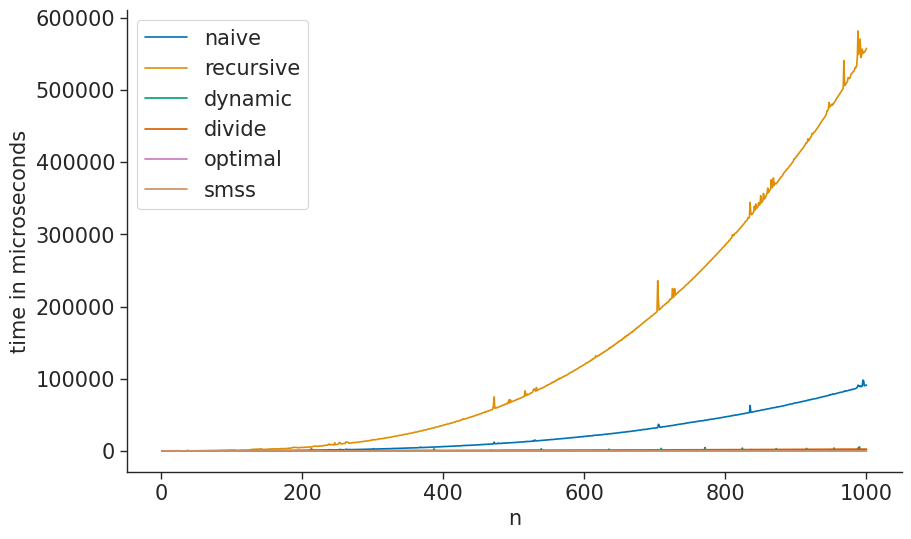
\includegraphics[width=0.8\textwidth]{../times_1000_all.png}
    \caption{Überblick aller Algorithmen für Eingabeintervall [1; 1000]}
    \label{fig:Ueberblick}
\end{figure}

\section{Aufgabe}

\subsection{2a - SMSS}\label{2a}
Wir erweitern den optimalen Ansatz, indem wir jedes gefundene \textit{segment} in einer \textit{ArrayList< ArrayList<int[3]> >} abspeichern.
Die äu\ss ere Liste initialisiert für jeden neuen \textit{max\_score} der gefunden wurde eine neue innere Liste. Diese innere
Liste wird so lange mit gleichwertigen \textit{segmenten} befüllt, bis ein \textit{segment} gefunden wurde, mit einen grö\ss erem
\textit{max\_score}. So ist die Liste von links nach rechts aufsteigend nach \textit{max\_score} sortiert (d.h. die letzte innere Liste beinhaltet alle \textit{MSS}).
Am Ende wird einmal über die am \textit{Endindex} stehende Liste in $\mathcal{O}(n)$ iteriert, um die tatsächlichen non overlapping
\textit{MSS} in einer finale Liste zu speichern.

Folgende Fälle werden abgedeckt: \\
\begin{verbatim} 
   CASE 1:
   1: ---+===+-----------
   2: ---+=====+---------
\end{verbatim}
Hier darf das $segment_{2}$ nicht ausgegeben werden, da $segment_{1} \subseteq segment_2$. Also merken wir uns
jeweils den Start- und Endindex des letzten \textit{segments}. So können wir die letzten Indizes mit den 
momentanen vergleichen und \textbf{CASE 1} abfangen. 

\begin{verbatim}
   CASE 2:
   1: ---+=====+---------
   2: ---+===+-----------
\end{verbatim}
\textbf{CASE 2} ist nicht möglich, da $segment_{2}$ vor $segment_{1}$ in der Liste abgespeichert ist.
Der Algorithmus ist so konzipiert, dass er wie bei \textbf{CASE 1} erst das kürzere $segment_{1}$ findet und dann das
längere $segment_{2}$. Also müssen wir uns nicht um \textbf{CASE 2} kümmern.
\begin{verbatim}
   CASE 3:
   1: -----+=+-----------
   2: ---+=====+---------

   CASE 4
   1: ---+=====+---------
   2: -----+=+-----------
\end{verbatim}
\textbf{CASE 3 \& 4} Sind ebenfalls nicht möglich, da \textit{MSS} entweder den gleichen Start- oder Endindex haben.

\begin{verbatim} 
   CASE 5:
   1: -----+===+---------
   2: ---+=====+---------
\end{verbatim}
Hier wird sich in der \textit{i-ten} Iteration die Start- und Endindizes von $segment_{1}$ gemerkt
und demnach das $segment_{2}$ in der \textit{i+1-ten} Iteration nicht dem Endresultat hinzugefügt,
da der Endindex von $segment_2 \not >$  Endindex von $segment_1$.
\subsection{2b - SMSS mit minimaler Länge}\label{2b}
\lipsum[1]
\subsection{2c - Alle MSS} 

Für die 2c haben wir unseren ursprünglichen Ansatz nicht weiter verwendet. Der \textit{optimale Algorithmus} ist in sich selbst so effizient,
dass er null Folgen am Anfang und am Ende von Segmenten direkt ignoriert. Wir haben uns also überlegt, welcher der anderen 
Algorithmen mit eine möglichst guten Laufzeit, diese Fälle auch betrachtet. Wir haben uns dazu entschieden den \textit{dynamic programming Algorithmus} zu erweitern. Dieser hat nämlich den Vorteil
bereits ohne Erweiterungen, alle Kombinationen von Teilintervallen zu betrachten. Insbesondere die Teilintervalle,
die der \textit{optimale Algorithmus} nicht in Betracht zieht.

\textbf{Beispiel}

\begin{verbatim}
                              5 -5 9 -3 13 -5 5 -5 5
      optimal             :   -----+=====+----------

      tatsächliche MSS    :   -----+=====+----------
                              -----+==========+-----
                              -----+===============+
                              +==========+----------
                              +===============+-----
                              +====================+
\end{verbatim}

\newpage
Der \textit{dynamic programming Algorithmus} betrachtet in dem oberen Beispiel alle der Teilfolgen. 
Also haben wir wieder wie in TODO eine äu\ss ere Liste mit inneren Listen erstellt, und für jeden neuen \textit{maxscore} eine neue innere Liste
erstellt, die dann mit allen gleichwertigen Segmenten (also allen Segmenten mit demselben \textit{maxscore}) befüllt wird, bis ein grö\ss erer \textit{maxscore} gefunden wird.
So findet der \textit{2\_c Algorithmus} also definitiv alle MSS, denn wir wissen bereits, dass der \textit{dynamic programming} Ansatz korrekt ist und
alle Kombinationen in Betracht zieht. Jedoch bu\ss t dieser Ansatz bei der Speicherkomplexität ein, das \textit{int[][]} Array wächst 
zu einem gegebenen Eingabe Vektor mit Länge $n$ exponentiell: $n^{2}$. D.h. für gro\ss e Eingaben verbrauchen wir enorm viel
Speicherplatz. 

Wie bereits in \textit{1. Theorie Blatt Aufgabe 2} gezeigt, benutzt der \textit{dynamic programming Algorithmus} immer nur 
die Hälfte des Arrays. Allgemein hat das Array die folgende Form:

$$
    \begin{pNiceMatrix}[left-margin]
    \times & \times & \times & \times & \times \\
           & \times & \times & \times & \times \\
           &        & \times & \times & \times \\ 
    \Block{2-2}<\Huge>{0}
           &        &        & \times & \times \\
           &        &        &        & \times \\
    \CodeAfter
     \tikz \draw (2-|1) -| (3-|2) -| (4-|3) -| (5-|4) -| (6-|5) ;
    \end{pNiceMatrix}
$$

\textbf{Beispiel}\\
 Betrachten wir die jeweiligen Endzustände der Datenstrukturen von Algorithmus \textit{2\_c} und der 
 Arbeitsspeicher schonenden Variante \textit{2\_c\_1}:
 \begin{itemize}
     \item Eingabe: $v = \left\{5, -5, 9, -3, 13, -5, 5, -5, 5\right\}$
     \item Hardware: (\textit{Processor: AMD® Ryzen 7 pro 4750u with radeon graphics × 16; Memory: 16.0 GB})
 \end{itemize}

\begin{verbatim}
 Array S[n][n] of Default Dynamic Programming (2_c) on v:
    0: [5 ,0 ,9 ,6 ,19,14,19,14,19]
    1: [0 ,-5,4 ,1 ,14,9 ,14,9 ,14]
    2: [0 ,0 ,9 ,6 ,19,14,19,14,19]
    3: [0 ,0 ,0 ,-3,10,5 ,10,5 ,10]
    4: [0 ,0 ,0 ,0 ,13,8 ,13,8 ,13]
    5: [0 ,0 ,0 ,0 ,0 ,-5,0 ,-5, 0]
    6: [0 ,0 ,0 ,0 ,0 ,0 ,5 , 0, 5]
    7: [0 ,0 ,0 ,0 ,0 ,0 ,0 ,-5,0 ]
    8: [0 ,0 ,0 ,0 ,0 ,0 ,0 ,0 ,5 ]
                               
 Max n on given Hardware: 30808:
 java -jar ... --algorithms 2_c --size 30808
\end{verbatim}

\begin{verbatim}
 ArrayList S containing int[] Arrays of Improved Dynamic Programming (2_c_1) on v:
    0: [5 ,0 ,9 ,6 ,19,14,19,14,19]
    1: [-5,4 ,1 ,14,9 ,14,9 ,14]
    2: [9 ,6 ,19,14,19,14,19]
    3: [-3,10,5 ,10,5 ,10]
    4: [13,8 ,13,8 ,13]
    5: [-5,0 ,-5,0]
    6: [5 ,0 ,5]
    7: [-5,0]
    8: [5]

 Max n on given Hardware: 44069:
 java -jar ... --algorithms 2_c_1 --size 44069
\end{verbatim}

Der \textit{improved dynamic programming 2\_c\_1} hat keine Position in der 
Datenstruktur, die ungenutzt bleibt. Der verbesserte Ansatz schafft es $13261$ zusätzliche
Zahlen zu verarbeiten, also ein $\approx 43\%$ grö\ss eres $n$ als der \textit{default 2\_c Algorithmus} 
(*auf der gegebenen Hardware). An der Komplexität hat sich durch die Abänderungen nichts geändert.
In Abbildung \ref{fig:time_comp_2c} werden die zwei Ansätze in ihrer Laufzeit verglichen.
Die Spikes in der Abbildung entstehen durch die inkonsistente Geschwindigkeit bei der Array Initialisierung.


\begin{figure}[t]
    \centering
    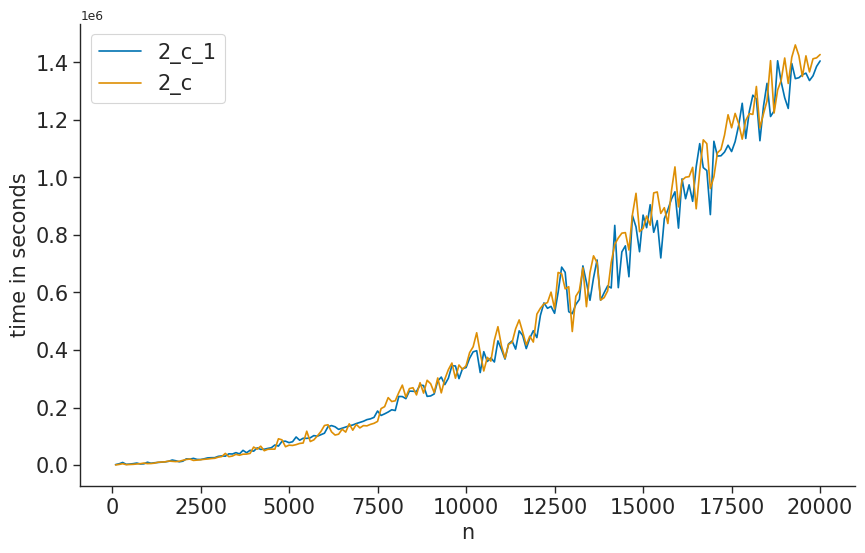
\includegraphics[width=0.8\textwidth]{../times_2c_20000.png}
    \caption{Ansatz 2\_c verglichen mit dem Arbeitsspeicher optimierten Ansatz 2\_c\_1}
    \label{fig:time_comp_2c}
\end{figure}



\newpage
\subsection{Ergebnisse}\label{performance_on_sheet_vec}
Um die  Ergebnisse auf dem Beispeil des Übungsblattes 
zu rekreiren ruft man die \textit{JAR} folgenderma\ss en auf:

\begin{verbatim}
java -jar JAR --v 5 -2 5 -2 1 -9 12 -2 24 -5 13 -12 3 -13 5 -2 -1 2

// Naive:
//
// 	[6,10] mit score 42
// 	466 µs
// 	for input size 19

// Recursive:
//
// 	[6,10] mit score 42
// 	180 µs
// 	for input size 19

// Dynamic Programming:
//
// 	[6,10] mit score 42
// 	29 µs
// 	for input size 19

// Divide and Conquer:
//
// 	[8,8] mit score 24
// 	847 µs
// 	for input size 19

// Optimal:
// 	[6,10] mit score 42
// 	4 µs
// 	for input size 19

// 2_a (MSS):
//
// 	[6,10] mit score 42
// 	24 µs
// 	for input size 19

// 2_b (SMSS):
//
// 	[6,10] mit score 42
// 	24 µs
// 	for input size 19

// 2_c (All SMSS):
//
// 	[6,10] mit score 42
// 	32 µs
// 	for input size 19

// 2_c_1 (All SMSS & Optimized space usage):
//
// 	[6,10] mit score 42
// 	49 µs
// 	for input size 19
\end{verbatim}

\end{document}
